\documentclass[xcolor=dvipsnames]{beamer}
\usetheme[navigation]{UMONS}
\usepackage[utf8]{inputenc}
\usepackage{graphicx}
\usepackage{wrapfig}
\usepackage{caption}
\usepackage{hyperref}
\usepackage{url}
\usepackage{color}
\usepackage{tikz}


\renewcommand{\arraystretch}{1.9}
\newcommand{\green}[1]{\textcolor{ForestGreen}{#1}}
\newcommand{\red}[1]{\textcolor{red}{#1}}

\title{Blockchain}
\author[G.Jérémy, D.Arman, L. Semih]{Gheysen Jérémy, Davidyan Arman, Locqueneux Semih}
\date{24 Avril 2018}
\institute[]{%
 Faculté des Sciences\\
  Université de Mons
  \\[2ex]
  
\includegraphics[height=4ex]{UMONS}\hspace{2em}%
  \raisebox{-1ex}{
\includegraphics[height=6ex]{UMONS_FS}}
}

\begin{document}

\maketitle

\section{Introduction}



\section{Smart Contract}

\begin{frame}{Smart Contract}
	
	
	\begin{center}
		Nick Szabo, \textit{Smart Contracts: Building Blocks for Digital Markets}, 1996
	\end{center}		
	
	\begin{figure}
		\centering
		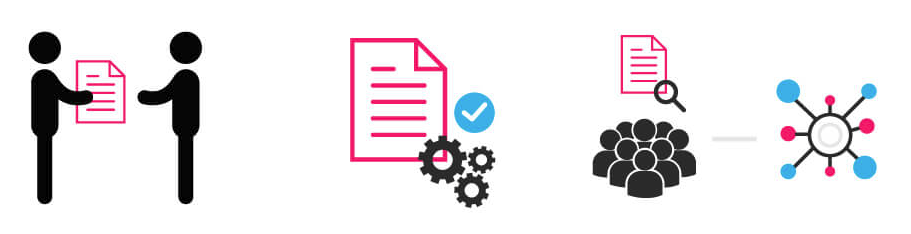
\includegraphics[scale=.25]{smart_contract}
		\caption{[Public domain]}
	\end{figure}
	
	
\end{frame}

\begin{frame}{Exemple d'Assurance}

	\begin{figure}
		\centering
		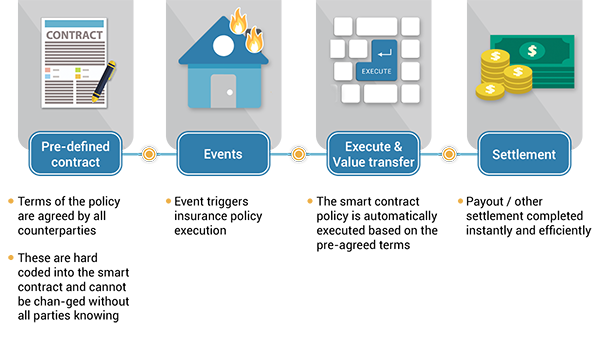
\includegraphics[scale=.5]{insurance_contract}
		\caption{By draglet GmbH [CC BY-SA 4.0 (https://creativecommons.org/licenses/by-sa/4.0)], from Wikimedia Commons}
	\end{figure}

\end{frame}

\begin{frame}{Exemple de code de contrat}

	\begin{figure}
		\centering
		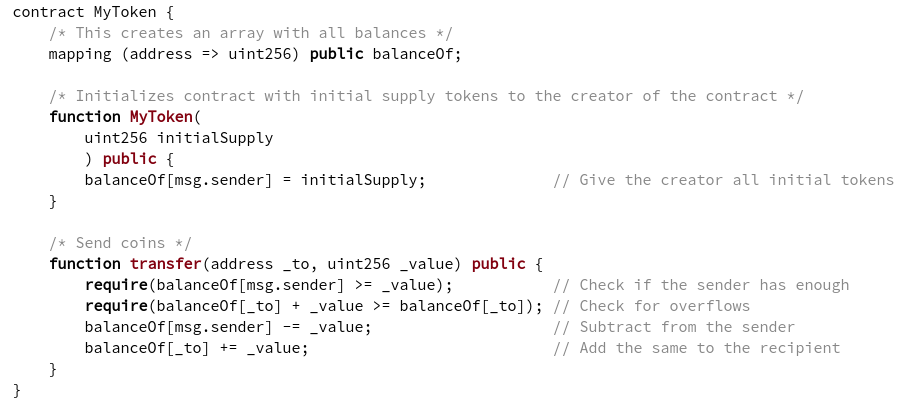
\includegraphics[scale=.35]{contract_example}
		\caption{An example smart contract on Ethereum. Source: https://www.ethereum.org/token}
	\end{figure}

\end{frame}

\begin{frame}{Ethereum Tokens}

	\begin{center}
		\color{blue}
		Smart Contract de Ethereum permet de créer des blockchains sur la base de leur blockchain
	\end{center}
	
	Exemple:
	\begin{figure}
	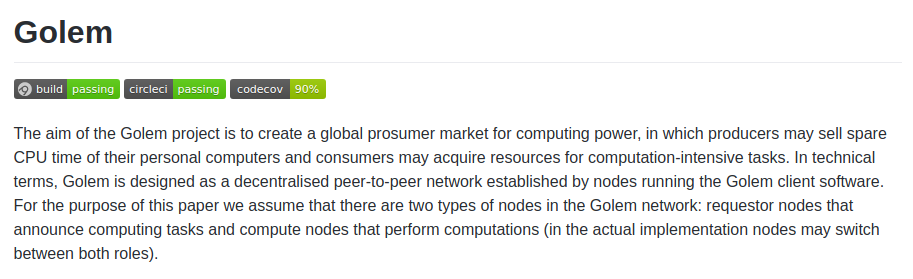
\includegraphics[scale=.35]{golem}
	\caption{source: page Github de Golem}
	\end{figure}

\end{frame}

\section{Conclusion}

\begin{frame}{Quelques Implementations Interessant de Blockchain}

	\begin{itemize}
		\item Estonie a completement digitalisé les données de leurs citvoyens.
		\item Regulation de Commerce des poisson grâce à Hyperledger Sawtooth.
		\item Testing de smart cities à Dubai.
		\item Des votes éléctornique à Moscou en 2014.
	\end{itemize}
	
\end{frame}

\end{document}